%\pagebreak
\section{Architecture}\label{sec:arch}

We now  give  an overview of   \system architecture.  We  discuss  the
design goals that    motivate  a new architecture, which     separates
functionality  into three different  planes,  architecture components,
and the mechanisms to achieve the design goals.
\subsection{Design Goals}

{\bf  Scalable   policy management.}    One   of  the  goals    of our
architecture is to ensure  that traffic is correctly forwarded through
a  middlebox chain according to network  policies.  Relying on routing
for traffic steering  is inefficient for  several reasons: distributed
routing protocols are slow to converge during topology reconfiguration
and   provide only  coarse-grained   control  over  flows.   SDN-based
solutions  avoid this problem  by installing per-flow rules on network
switches, but these do not scale well since the SDN controller must be
involved  on per-flow decisions, and switches  have  limited memory to
store flow rules; in the worst case, each switch must install one rule
per TCP flow.

In \system,    we avoid both of    these scalability  impediments. The
protocol is designed such that the destination  address of each packet
identifies the next middlebox  or endpoint in  the path and the source
address identifies the sending  middlebox or endpoint. Doing so avoids
the need of routing tweaks  when network topology changes or endpoints
move.    Policy  management in \system  is   controlled by a logically
centralized controller,  but  packets  on the   data  plane are  never
redirected  to the policy server.   This is a  key difference from SDN
solutions  that queue packets  on the controller during flow migration
between middleboxes~\cite{OpenNF}.   Moreover, the  policy  server can
delegate per-flow  decisions   to the middleboxes.   For   instance, a
middlebox  may autonomously  decide to remove  itself  from  a session
path. Delegation further relaxes any dependence on the policy server.

{\bf   Low  performance overhead.}   Recall    that we  identify  each
connection  with a   supersession and  its   associated subsessions. A
simple approach for decomposing a supersession into subsessions can be
implemented by establishing  tunnels between middeboxes.   However, in
adding a  new  header  to   each  packet,  this  approach   introduces
significant  overhead   from MTU  increase    and consequently  packet
fragmentation. Packet fragmentation  can  be solved by  increasing the
MTU of switches  and routers inside  a single  network administration,
but this  solution is not  viable when packets  have  to cross network
domains,  which   has become  a  common   case in virtualized  network
functions that are outsourced to  public clouds.  Moreover,  solutions
that rely on tunnels generally add extra  overheads such as encryption
and compression~\cite{Aplomb}, features  that  might be   redundant or
unnecessary  to   all   flows.  \system   relies   on network  address
translation for explicitly  addressing subsession endpoints, hence the
only overhead is incurred by  port remapping.  Also, supersession  IDs
in \system are not carried on each  packet, as in~\cite{DOA}. They are
stored   on the   middlebox   agents  during  supersession   setup  or
supersession reconfiguration during middlebox migration.

{\bf  Endpoint  mobility and  NF   migration.}  
%\amy{How  about  renaming    this   sub point    as   ``Separation  of 
%  Functionality'', or   something  that references the   separation of
%  decision-making into 3 planes, or  even something about  simplicity.
%  Separating planes so that  you  can cleanly implement  host mobility
%  and NF migration. In any case, the current title is meaningless.}
The growing trend in network function virtualization can cause dynamic
migration of flows between  middleboxes. Along with frequent  end host
location changes  due to device mobility  or  VM migration,  these new
possibilities  complicate     traffic-steering  solutions  relying  on
administrative control over network routing.  In \system architecture,
a  separate policy  server decides  (i)   the sequence of  middleboxes
traffic should traverse and  (ii) informs the hosts--whether endpoints
or  middleboxes--of these decisions by pushing  policies ahead of time
to avoid increasing connection set-up  delay.  Then, the policy server
steps back  and allowing these  hosts to establish sessions and handle
migrations as needed.

% Incremental deployment
% This will be moved to a different subsection
% 1. Does not rely on a special  naming infrastructure. It can use any
% scheme,  as  long as   the   endpoints can   be  identified  in  the
% subsessions. A different naming scheme, however, requires applications
% and NFs changes.
% 2.  Does not require all the   components to be  integrated into the
% architecture for initial deployment. 
% 3. Does not require application or NF changes.

\subsection{Components}

An overview of  the \system architecture  with its main components and
the    interactions     between   the    modules    is    depicted  in
Figure~\ref{architecture}.   The  architecture     presents    a clear
separation of  management,  control, and  data planes functionalities.
The management  plane   is composed   of  a   policy server that    is
responsible for coordinating the agents on  the control plane based on
high-level network policies provided by the network administrator. The
control  plane implements   the protocol  in  \S\ref{sec:protocol} for
session initiation, flow migration, and network function insertion and
removal.   The data plane is  responsible for translating supersession
IDs  into local IP addresses    and ports, delivering  packets to  the
network functions,  and forwarding   packets between  middleboxes.  To
simplify  the presentation, we first  assume a homogeneous scenario in
which endpoints  and all middleboxes run \system  agents, and defer to
\S\ref{sec:discussion} a discussion of a more realistic scenario where
\system  can be deployed incrementally.  Also,  we assume that network
functions  do  not   change  the  packet  5-tuple  (i.e.,   source and
destination IP addresses  and  port numbers,  and protocol type),  the
case    where     packets  are   changed    will    be   discussed  in
\S\ref{sec:NFsupport}.

\begin{figure}[hb]
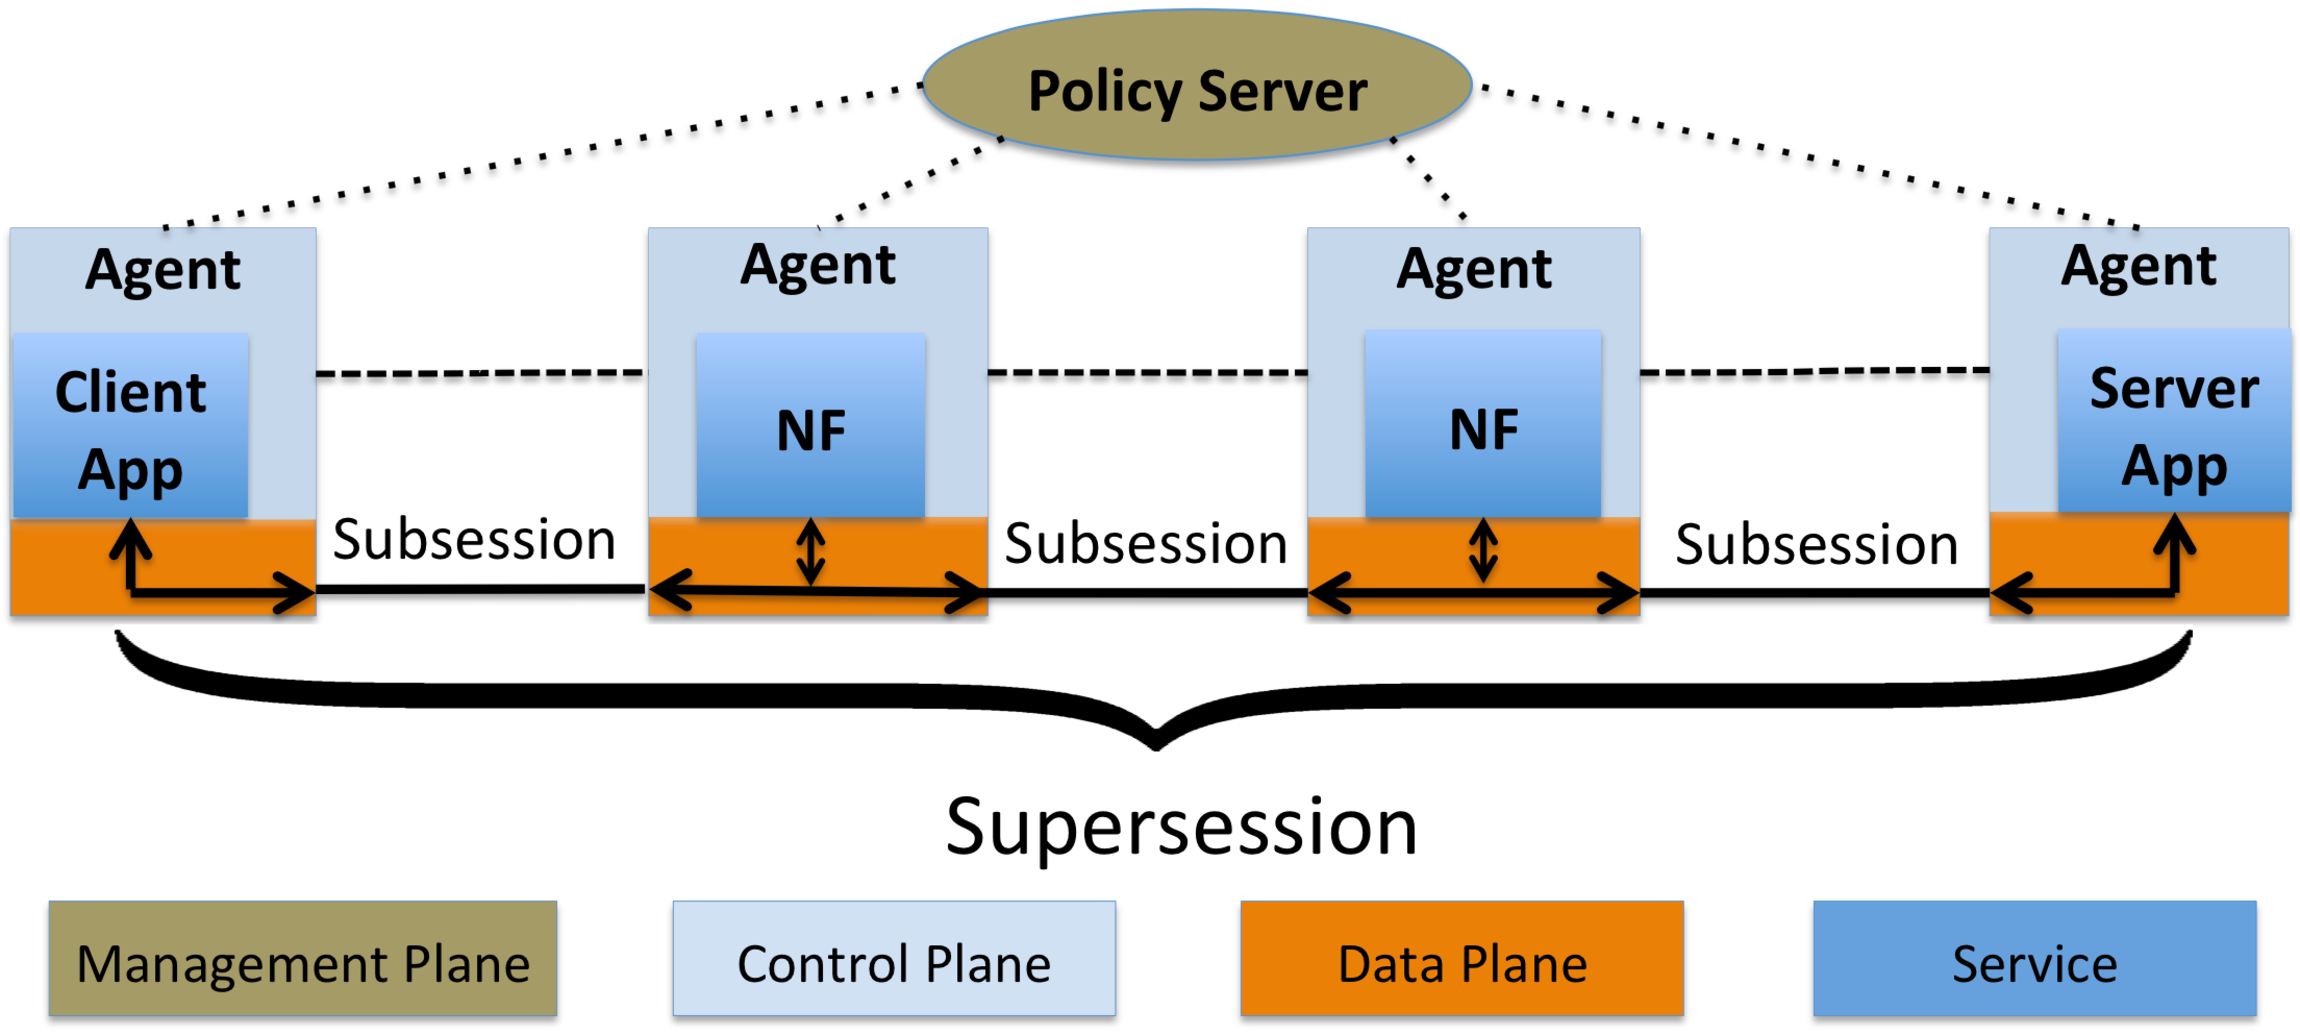
\includegraphics[width=\linewidth]{figures/archi.pdf}
\caption{\small\system architecture}\label{architecture}
\end{figure}

% Load   balancing:    Due to the    complex   packet  processing that
% middleboxes run  (e.g.,  deep packet  inspection),  a key  factor in
% middlebox deployments   is to balance the   processing load to avoid
% overload.

% To avoid inference algorithms, which  do not give 100 precision,  we
% may require  NF modifications so they  can interact with the \system
% agents.

% Typical middlebox policies require a packet (or session) to traverse
% a sequence of middlebox (This is  an instance of the broader concept
% of "service chaining").  In our example,  the administrator wants to
% route all HTTP traffic through the policy chain FW-IDS-PROXY and the
% remaining  traffic   through  the   chain FW-IDS.  Note   that  many
% middleboxes  are stateful and need to  process  both directions of a
% session for correctness.

% Middlebox resource management:  Studies show that middlebox overload
% is a  common cause of failures.  

% "The  policy server can take global   decisions to avoid overload or
% give multiple options to the \system agents  so they can balance the
% load across their neighbors.

% SIMPLE 

{\bf Policy  server:}   The  \system  policy  server is   a  logically
centralized server that receives  high-level policy specification from
the  network  administrator and reliably   delivers subpolicies to the
agents, i.e., it makes sure that an agent receives a policy consistent
with its location.  For instance,  a client agent should receive  only
policies related to the network it is connected.

The  policy server makes  global decisions based on: (i) configuration
changes  or (ii)   network state changes.    Configuration changes are
triggered  by the network administrator and  network state changes are
triggered  by monitoring   information.  The  policy  server  receives
monitoring  information  from the \system   agents and  may  decide to
migrate flows   from an overloaded   network function to   a different
instance, insert new network functions  in a supersession (e.g., a DPI
may be dynamically introduced after  a light IDS detects that  packets
from  a  supersession  need deeper  inspection), or   remove a network
function  out of a  supersession path because it  is no longer needed.
However, the   policy  server does  not need  to  be  involved  in all
fine-grained decisions, it can offload decisions to the \system agents
runing on the middleboxes as determined  by the network administrator.
A common decision that  can be easily offloaded to  the agents is  the
selection   of a     network   function instance   when  the   network
administrator configures multiple instances of the same type.

%The policy server also decides how a supersession is It determines how
%a supersession is initially divided into subsessions, i.e., it decides
%the middlebox chain a set of flows should traverse in order to enforce
%a network policy.

%- It outsources fine grain  decisions to the  middlebox agents. It can
%send to the middlebox agents a list of MB types to  from the MB chain,
%but the decision to pick an instance is outsourced to  the MBA. It can
%also provide autonomy to a MB to remove itself out the way of a flow.

In  \system,  policies define the service  chains  to be  traversed by
different packets  or sessions (e.g.,  packets from subnet 10.0.1.0/24
should    be     forwarded       through      the     chain     \{Load
Balancer$\rightarrow$IDS$\rightarrow$Firewal$\rightarrow$Proxy\}).   A
policy  specifies a  predicate,  which is  used  to restrict  a set of
packets, and a  sequence of network  function types.  The general form
of a policy is:
\begin{center}
{\tt match(predicate) >> \{NFT$_1 \rightarrow\cdots\rightarrow$ NFT$_n$\}}
\end{center}
%\noindent where
%\begin{center}
%{\tt NFT$_i$ = \{Set of IP addresses\}}
%\end{center}
A predicate is specified with source and  destination IP addresses and
ports, and protocol types.   Complex predicates can be specified using
conjunction (\&),  disjunction  ($|$),  and negation (\~{})  operators
like in Pyretic~\cite{pyretic}. A packet that satisfies  the predicate in the
match  statement is forwarded  through  the chain of network  function
types specified  on the right-hand side of  the  {\tt >>} operator.  A
network   function type ({\tt NFT$_i$})   specifies  a set of  network
function instances  of the same  type.  The network  administrator can
specify, for example, a set with the IP addresses of proxy servers and
the policy  server can choose an  instance for sessions initiated in a
specific  client or  it  can delegate   this  decision to  the \system
agents.

%Predicates: The  predicates are specified  with respect to the point a
%packet enters  the  network,  i.e., the  point  of attachment    of an
%endpoint.


{\bf \system Agents:} \system  agents  are key components to   enforce
network  policies.   They  must  ensure  that   packets are  correctly
forwarded  to the next  middlebox on the  service chain  or dropped if
they  do  not  comply with  the network   policy.   Whenever  a client
application starts a connection, the \system agent running on the same
machine intercepts  the first packet of the  connection and matches it
with  the client's   network  policies to   determine the  sequence of
network function types  the packet must be  forwarded.  If  a match is
found, the  agent starts the  session  setup protocol in \S\ref{setup}
that will  create    the  subsessions between   middleboxes  and   the
corresponding  mappings between incoming and  outgoing packets in each
middlebox on the session path.   The 5-tuple of the client  connection
is used  to identify the supersession  packets when they are processed
by   the network functions.   Once   the  supersession  is  setup, all
subsequent  packets from the  client's connection are forwarded to the
first middlebox on the service chain.

In each middlebox, a  \system agent must  create two mappings for each
session. One, which we call horizontal NAT,  translates the 5-tuple of
an incoming  packet to the corresponding 5-tuple  that is  used in the
next   subsession.  The   other one,  which   we  call vertical   NAT,
translates   the 5-tuple of each   incoming packet to the supersession
5-tuple before the  packet is delivered to the  network function or to
the applications on  the  endhosts.  Keeping the  supersession 5-tuple
invariant    on  the middleboxes  has  a    few advantages. First,  it
simplifies policy specification, because the network administrator can
design policies based only on the  endpoint addresses without worrying
about  the subsessions.  Second,  it simplifies network function state
migration, because network functions  always receive packets  with the
supersession  5-tuple   regardless of flow    migrations or  middlebox
insertions  or removals.  Third,  network functions that do not change
the packet 5-tuple do not need to be changed to work with \system.

\system agents are also heavily involved  on service chain maintenance
and  supersession  reconfigurations.   The  agents report   management
information, such as resource utilization  in the middleboxes, to  the
policy server, so  it  can  take  global management  decisions   about
service chains.  Reconfigurations can  also be triggered by a  network
function,  if allowed  by  the network  policy.   A  common case  of a
reconfiguration triggered by a network function is  when a cache proxy
detects that the content of a session is not cacheable and signals the
\system agent to  remove the  proxy  from the service  chain.  Once  a
reconfiguration is  initiated, either by the policy   server or by the
network function,  \system      agents  execute the  protocols      in
\S\ref{MigrateLogic}.

%{\bf End hosts:}

%\subsection{Division of Labor}

%Clean separation of control, data, and management 

%\subsection{Mechanisms}

